


\tikzset{every picture/.style={line width=0.75pt}} %set default line width to 0.75pt        

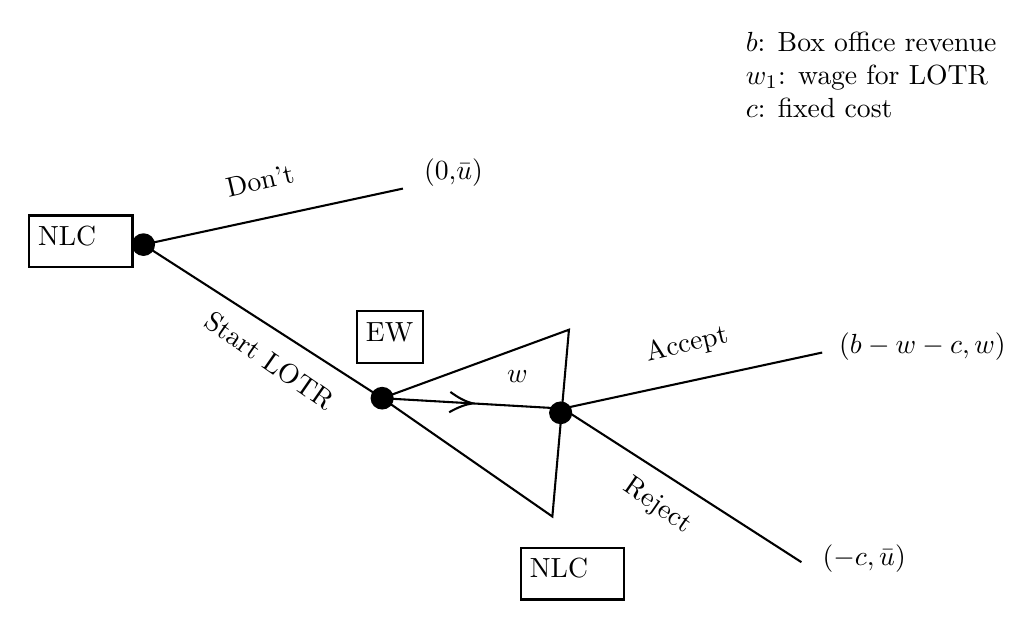
\begin{tikzpicture}[x=0.75pt,y=0.75pt,yscale=-1,xscale=1]
%uncomment if require: \path (0,313); %set diagram left start at 0, and has height of 313

%Straight Lines [id:da08747788290842107] 
\draw    (91.29,121.02) -- (206.29,195.02) ;
%Straight Lines [id:da20945690928904903] 
\draw    (216.29,94.02) -- (91.29,121.02) ;
%Shape: Polygon [id:ds13296135404903886] 
\draw   (296.29,162.02) -- (296.29,162.02) -- (288.29,252.02) -- (288.29,252.02) -- (206.29,195.02) -- cycle ;
%Straight Lines [id:da9208510134743559] 
\draw    (206.29,195.02) -- (293.29,200.02) ;
\draw [shift={(249.79,197.52)}, rotate = 183.29] [color={rgb, 255:red, 0; green, 0; blue, 0 }  ][line width=0.75]    (10.93,-4.9) .. controls (6.95,-2.3) and (3.31,-0.67) .. (0,0) .. controls (3.31,0.67) and (6.95,2.3) .. (10.93,4.9)   ;
%Straight Lines [id:da2678361360716295] 
\draw    (293.29,200.02) -- (408.29,274.02) ;
%Straight Lines [id:da39036490074799657] 
\draw    (418.29,173.02) -- (293.29,200.02) ;
%Shape: Ellipse [id:dp4460632558797326] 
\draw  [fill={rgb, 255:red, 0; green, 0; blue, 0 }  ,fill opacity=1 ] (201.22,195.02) .. controls (201.22,192.28) and (203.49,190.06) .. (206.29,190.06) .. controls (209.09,190.06) and (211.36,192.28) .. (211.36,195.02) .. controls (211.36,197.76) and (209.09,199.98) .. (206.29,199.98) .. controls (203.49,199.98) and (201.22,197.76) .. (201.22,195.02) -- cycle ;
%Shape: Ellipse [id:dp5183488462286219] 
\draw  [fill={rgb, 255:red, 0; green, 0; blue, 0 }  ,fill opacity=1 ] (287.22,202.06) .. controls (287.22,199.32) and (289.49,197.1) .. (292.29,197.1) .. controls (295.09,197.1) and (297.36,199.32) .. (297.36,202.06) .. controls (297.36,204.8) and (295.09,207.02) .. (292.29,207.02) .. controls (289.49,207.02) and (287.22,204.8) .. (287.22,202.06) -- cycle ;
%Shape: Ellipse [id:dp9043754387347656] 
\draw  [fill={rgb, 255:red, 0; green, 0; blue, 0 }  ,fill opacity=1 ] (86.22,121.02) .. controls (86.22,118.28) and (88.49,116.06) .. (91.29,116.06) .. controls (94.09,116.06) and (96.36,118.28) .. (96.36,121.02) .. controls (96.36,123.76) and (94.09,125.98) .. (91.29,125.98) .. controls (88.49,125.98) and (86.22,123.76) .. (86.22,121.02) -- cycle ;

% Text Node
\draw (128.41,88.18) node [anchor=north west][inner sep=0.75pt]  [rotate=-346.86] [align=left] {Don't};
% Text Node
\draw (124.59,150.54) node [anchor=north west][inner sep=0.75pt]  [rotate=-34.76] [align=left] {Start LOTR};
% Text Node
\draw (225,78) node [anchor=north west][inner sep=0.75pt]   [align=left] {(0,$\bar u$)};
% Text Node
\draw    (36,107) -- (86,107) -- (86,132) -- (36,132) -- cycle  ;
\draw (39,111) node [anchor=north west][inner sep=0.75pt]   [align=left] {NLC};
% Text Node
\draw (265,180) node [anchor=north west][inner sep=0.75pt]   [align=left] {$w$};
% Text Node
\draw (330.41,167.18) node [anchor=north west][inner sep=0.75pt]  [rotate=-346.86] [align=left] {Accept};
% Text Node
\draw (326.59,229.54) node [anchor=north west][inner sep=0.75pt]  [rotate=-34.76] [align=left] {Reject};
% Text Node
\draw    (194,153) -- (226,153) -- (226,178) -- (194,178) -- cycle  ;
\draw (197,157) node [anchor=north west][inner sep=0.75pt]   [align=left] {EW};
% Text Node
\draw    (273,267) -- (323,267) -- (323,292) -- (273,292) -- cycle  ;
\draw (276,271) node [anchor=north west][inner sep=0.75pt]   [align=left] {NLC};
% Text Node
\draw (425,162) node [anchor=north west][inner sep=0.75pt]   [align=left] {$(b-w-c,w)$};
% Text Node
\draw (417,264) node [anchor=north west][inner sep=0.75pt]   [align=left] {$(-c,\bar u)$};
% Text Node
\draw (380,17) node [anchor=north west][inner sep=0.75pt]   [align=left] {$b$: Box office revenue\\$w_1$: wage for LOTR\\$c$: fixed cost };


\end{tikzpicture}